\documentclass[tikz,border=2pt]{standalone}
\usepackage{tikz}
\usetikzlibrary{positioning,arrows.meta}

\begin{document}
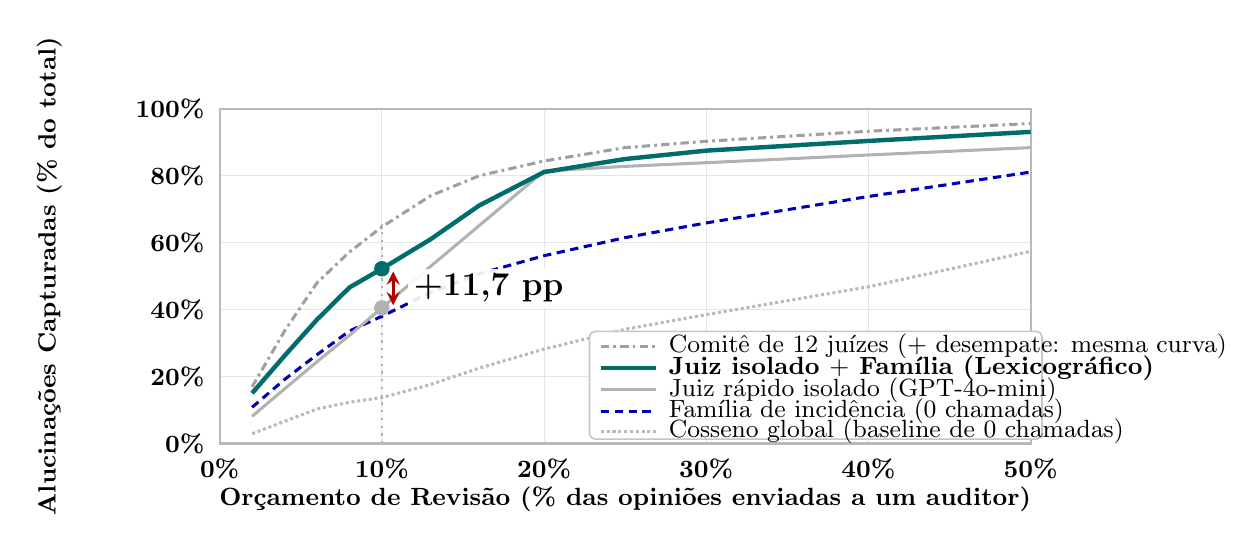
\begin{tikzpicture}[x=0.206cm, y=0.0425cm, font=\small,
                    c/.style={line width=1.1pt, line join=round},
                    comite/.style={c, gray!75, dash pattern=on 3pt off 1.5pt on 1pt off 1.5pt},
                    jlex/.style={c, line width=1.6pt, color=teal!85!black},
                    juiz/.style={c, gray!60},
                    fam/.style={c, densely dashed, color=blue!70!black},
                    cosg/.style={c, gray!55, densely dotted}]
  \draw[gray!20] (0,0) grid[xstep=10, ystep=20] (50,100);
  \draw[gray!55, line width=0.8pt] (0,0) rectangle (50,100);
  \foreach \x in {0,10,20,30,40,50} \node[below=2pt] at (\x,0) {\textbf{\x\%}};
  \foreach \yy in {0,20,40,60,80,100} \node[left=2pt] at (0,\yy) {\textbf{\yy\%}};
  \node[below=12pt] at (25,0) {\textbf{Orçamento de Revisão (\% das opiniões enviadas a um auditor)}};
  \node[rotate=90] at (-10.5,50) {\textbf{Alucinações Capturadas (\% do total)}};
  \draw[gray!60, dotted, line width=0.8pt] (10,0) -- (10,66);
  \draw[cosg] plot coordinates {(2,2.9) (4,6.6) (6,10.3) (8,12.3) (10,13.7) (13,17.6) (16,22.5) (20,28.2) (25,34.1) (30,38.5) (40,46.8) (50,57.4)};
  \draw[fam] plot coordinates {(2,10.8) (4,19.1) (6,26.5) (8,33.6) (10,38.0) (13,45.1) (16,50.7) (20,56.1) (25,61.5) (30,65.9) (40,73.8) (50,81.1)};
  \draw[juiz] plot coordinates {(2,8.1) (4,16.3) (6,24.4) (8,32.3) (10,40.5) (13,52.9) (16,65.1) (20,81.4) (25,82.8) (30,83.9) (40,86.2) (50,88.4)};
  \draw[jlex] plot coordinates {(2,15.0) (4,26.2) (6,37.0) (8,46.6) (10,52.2) (13,61.0) (16,71.1) (20,81.1) (25,85.0) (30,87.5) (40,90.4) (50,93.1)};
  \draw[comite] plot coordinates {(2,16.9) (4,33.6) (6,48.0) (8,57.2) (10,64.7) (13,74.0) (16,80.0) (20,84.4) (25,88.4) (30,90.3) (40,93.3) (50,95.6)};
  \fill[teal!85!black] (10,52.2) circle (2.8pt); 
  \fill[gray!60] (10,40.5) circle (2.8pt);
  \draw[<->, >=stealth, line width=1.1pt, red!70!black] (10.7,41.3) -- (10.7,51.4);
  \node[anchor=west, inner sep=2pt, fill=white, fill opacity=0.9,
        text opacity=1] at (11.6,46.3) {\textbf{\large +11,7 pp}};
  % legend
  \begin{scope}[shift={(23.5,2.5)}]
    \draw[fill=white, draw=gray!45, rounded corners=2pt, line width=0.6pt] (-0.7,-1.2) rectangle (27.2,31);
    \draw[comite] (0,26.5) -- (3.4,26.5);
      \node[anchor=west, inner sep=1.5pt] at (3.9,26.5) {Comitê de 12 juízes ($+$ desempate: mesma curva)};
    \draw[jlex]   (0,20.0) -- (3.4,20.0);
      \node[anchor=west, inner sep=1.5pt] at (3.9,20.0) {\textbf{Juiz isolado $+$ Família (Lexicográfico)}};
    \draw[juiz]   (0,13.5) -- (3.4,13.5);
      \node[anchor=west, inner sep=1.5pt] at (3.9,13.5) {Juiz rápido isolado (GPT-4o-mini)};
    \draw[fam]    (0,7.0) -- (3.4,7.0);
      \node[anchor=west, inner sep=1.5pt] at (3.9,7.0) {Família de incidência (0 chamadas)};
    \draw[cosg]   (0,1.2) -- (3.4,1.2);
      \node[anchor=west, inner sep=1.5pt] at (3.9,1.2) {Cosseno global (baseline de 0 chamadas)};
  \end{scope}
\end{tikzpicture}
\end{document}
